\section{Entropy}
Entropy is central to the second and third laws of thermodynamics, as well as understanding the spontaneity of processes. It's a concept you'll see appear not only in physics, but in chemistry and biology as well.

\subsection{Types of Systems}
Just before we define our notion of this mysterious "entropy", it will help to define what different kinds of systems mean. An \textbf{Open system} is one in which both matter and energy can be exchanged with its environment. A \textbf{Closed system} is a system where energy can be exchanged with the environment, but no matter. Finally, an \textbf{isolated} system is where neither matter nor energy can be exchanged with the environment. \\
As a quick example, suppose my system is a half cup of water. If I leave the top of the cup open, it's an open system as the water molecules can evaporate and leave the cup. If I close the top of the cup, then it's a closed system as I can still give energy to the cup (say, by heating it in a microwave) even if the water molecules can't escape from it. If the cup is perfectly insulated and closed off, then its an isolated system as neither matter nor energy can enter or exit the cup. With this in mind, let's proceed with the most mindbending concept of this unit!
\subsection{The Classical Definition of Entropy}
Jumping right into things, entropy, for large systems, can be defined as
\begin{equation}
    dS=\frac{\delta Q_{rev}}{T}
\end{equation}
Where $dS$ is the change in entropy, $\delta Q_{rev}$ is heat reversibly flowing to/from a system, and $T$ is the temperature of the system. Just stating it right here, this equation probably seems to make \textbf{no} sense whatsoever, so let's step back a bit to build up to it.
\subsubsection{Reversable Processes}
First we need to talk about reversible processes. A reversible process, broadly speaking, is one that can spontaneously take place in both directions. Let's take a look at an example: say we have two large closed chambers of gas in an isolated system. The only way they can interact is via heat flow.
\begin{figure}[h!]
    \centering
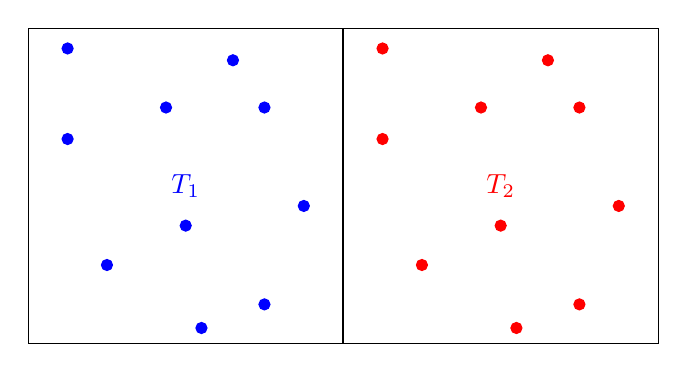
\begin{tikzpicture}
\draw[draw = black] (0,0) rectangle (8,4);
\draw[thick] (4,0) -- (4,4);
\draw[text=blue] (2,2) node {$T_1$};
\draw[text=red] (6,2) node {$T_2$};
\draw[fill=blue, draw=blue] (1,1) circle (2pt);
\draw[fill=blue, draw=blue] (3,0.5) circle (2pt);
\draw[fill=blue, draw=blue] (0.5,2.6) circle (2pt);
\draw[fill=blue, draw=blue] (2.6,3.6) circle (2pt);
\draw[fill=blue, draw=blue] (3.5,1.75) circle (2pt);
\draw[fill=blue, draw=blue] (1.75,3) circle (2pt);
\draw[fill=blue, draw=blue] (2,1.5) circle (2pt);
\draw[fill=blue, draw=blue] (2.2, 0.2) circle (2pt);
\draw[fill=blue, draw=blue] (3,3) circle (2pt);
\draw[fill=blue, draw=blue] (0.5, 3.75) circle (2pt);
\draw[fill=red, draw=red] (5,1) circle (2pt);
\draw[fill=red, draw=red] (7,0.5) circle (2pt);
\draw[fill=red, draw=red] (4.5,2.6) circle (2pt);
\draw[fill=red, draw=red] (6.6,3.6) circle (2pt);
\draw[fill=red, draw=red] (7.5,1.75) circle (2pt);
\draw[fill=red, draw=red] (5.75,3) circle (2pt);
\draw[fill=red, draw=red] (6,1.5) circle (2pt);
\draw[fill=red, draw=red] (6.2, 0.2) circle (2pt);
\draw[fill=red, draw=red] (7,3) circle (2pt);
\draw[fill=red, draw=red] (4.5, 3.75) circle (2pt);
\end{tikzpicture}
    \caption{The wonderful box with two closed sections.}
\end{figure}
\\ If one side is at a higher temperature than the other, then we intuitively know that heat will flow from the hot side to the cool side. But what happens if their temperatures are the same? The short answer is: absolutely nothing. But it's an exciting nothing! Let's dig even deeper. \\
\newline
Say we were to zoom in extremely close on that boundary between the two sides of the box. What would we see? Unsurprisingly, a lot of very small particles hitting a very large wall. However, we know that in order for heat to flow across that barrier, the particles need some way of transferring their energy across the wall. How could they do it? Well, there's two possible ways. The first is radiation, which we'll pretend doesn't exist (it makes our lives much easier, and isn't a terrible assumption). The other is through the wall itself. That is, when a particle collides with the wall, a bit of its kinetic energy goes into the wall, which then gives it up to a particle colliding on the other side.
\newline\newline
Here's the key though: particles on both sides of the wall do this, regardless of the temperature difference. Even if we had the right side of the box at $10^{20}\mathrm{K}$ \footnote{Actually at a temperature this high there would be no box.} and the left side at $100\mathrm{K}$, some particles from the left side of the box would hit the wall and give up some energy to the right side. It's just that particles on the right side of the box are
\begin{enumerate}
    \item Giving up way more energy when they hit the wall.
    \item Hitting the wall far more frequently.
    \item And/or both!
\end{enumerate}
So the \textit{net} transfer of energy is from the right side of the box to the left. In a situation like this, where there is a spontaneous net transfer of energy, we'd say that said process is irreversible. However, if the temperature in the box was the same at both sides, we'd expect no net heat transfer to take place. Therefore, we could conclude that
\begin{itemize}
    \item Both sides give up the same amount of energy per collision on average.
    \item Both sides have the same frequency of collision.
\end{itemize}
This is where the symbol $\delta$ comes in. As the profs may or may not have mentioned in lecture, it means a \textit{very very very} small change. Which, it so happens, is the perfect way to describe the change in energy/temperature each side of the box has when one collision occurs. So we have a very small heat flow, and essentially constant temperature. Furthermore we can see that this tiny flow of heat has an equal chance of happening in both directions, and will. Hence, its reversible!
\newline\newline
So now that we have a better idea of what a reversible process is, we can better understand what entropy is. As a quick reminder, we said above that
\begin{equation*}
    dS=\frac{\delta Q_{rev}}{T}
\end{equation*}
With our newfound knowledge we can say that this says: the change in entropy of a system ($dS$) in a \textit{reversible} heat transfer is \textit{directly} proportional to the amount of heat transferred into the system and \textit{inversely} proportional to the temperature of the system.\footnote{Some of you may wonder if this definition still can be applied when the heat transfer is irreverisible. It can, but the equality is replaced by in inequality $dS > \frac{dQ}{T}$. So if you wanted the most general definition would be $dS \geq \frac{dQ}{T}$.}
\newline\newline
We say above that our tiny reversible processes happen between two systems at the same (constant) temperature. Here's the issue though, and the one that causes us to define all our reversible processes (and entropy) as infinitesimals: no reversible process actually exists on a macroscopic scale.
\newline\newline
As an example of why this is, let's take a look at a process that is theoretically reversible, but isn't actually reversible. Say we have a container of a gas with a piston on one face, but insulated such that it cannot exchange heat (or molecules) with its environment. However, it is connected to a neighbouring infinitely large heat bath, where it can exchange heat with (but not molecules). 
\begin{figure}[h!]
\centering
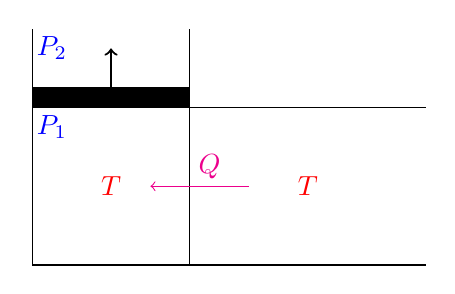
\begin{tikzpicture}
\draw[draw=black] (0,0) rectangle (2,2);
\draw[fill = black] (0,2) rectangle (2,2.25);
\draw (0,2) -- (0,3);
\draw (2,2) -- (2,3);
\draw (2,2) -- (5,2);
\draw (2,0) -- (5,0);
\draw[->, thick] (1, 2.25) -- (1, 2.75);
\draw[text=blue] (0.25,1.75) node {$P_1$};
\draw[text=blue] (0.25, 2.75) node {$P_2$};
\draw[text=red] (1,1) node {$T$};
\draw[text=red] (3.5,1) node {$T$};
\draw[magenta, ->] (2.75,1) -- (1.5,1);
\draw[text=magenta] (2.25, 1.25) node {$Q$};
\end{tikzpicture}
\caption{Piston with infinite heat bath to the right.}
\end{figure}
In this situation, we have that $P_{1}>P_{2}$, so the piston will undergo an expansion. Since the heat bath beside it will keep it at the same temperature, the expansion will be isothermal. So since the temperature of the two sides of the piston/heat bath barrier is constant and equal, the heat transfer across it reversible right? Well, not quite. And it has to do with the idea that a perfectly isothermal process doesn't exist either.
\newline\newline
To figure out why, let's break down what happens step by step. Initially, both the gas and the heat bath are at the same temperature, so no net heat flow between them. However, the pressure inside the piston is greater than the pressure outside. So the piston expands. When it does this, it does work on the environment, and loses energy. This in turn causes its temperature to fall. Its temperature dropping causes heat to flow spontaneously across from the heat bath, until the gas returns to its original temperature. Rinse, repeat until the internal and external pressures are equal.
\newline\newline
So we can see that during an isothermal process, the temperature isn't quite constant. However, if we do this process \textit{very} slowly, the heat flow will manage to restore the temperature so quickly (or to put it another way, heat will flow into the system much faster than the system does work) that the temperature be \textit{almost} constant the whole time. This is what we really mean by an isothermal process. It's also why entropy is defined infinitesimally, since we approximate that each of our tiny expansion steps of the piston happen at constant temperature.
\newline\newline
That being said, imagining an ideal, isothermal process is extremely useful, especially at small time scales. It allows us to derive the following formula for the change in entropy:
\begin{equation}
    \label{eqn:(36)}
    \Delta S=n{c_{v}}\ln{\frac{T_1}{T_0}} + nR\ln{\frac{V_1}{V_0}}
\end{equation}
Here, $n$ is the number of mols of gas, $c_v = \frac{\chi}{2}R$ as we defined earlier (for $\chi$ degrees of freedom and the gas constant $R$), $T_0$ and $T_1$ are the initial and final temperatures, and $V_0$ and $V_1$ are the initial and final volumes. First, the change in entropy depends only on the initial and final states of the system (i.e. the final and initial temperatures and volumes), not the path between those states! So \textbf{entropy is function of state}.
\newline\newline
The second thing you should notice is that entropy of a system is dependent on the volume, an \textit{extensive} quantity. Therefore, \textbf{entropy is an extensive quantity}.

\subsubsection{(Optional) Derivation of the Sackur–Tetrode Equation}
Equation \ref{eqn:(36)} as shown above is actually a version of the Sackur-Tetrode equation, which gives the entropy of a monoatomic ideal gas in full. While the derivation of the full equation is far, far out of the scope of this course\footnote{You may consult Wikipedia if you want to see the full equation}, equation \ref{eqn:(36)} can totally be derived with the things we have learned. This derivation is more for your curiousity than anything, and you do already have all the tools required to derive it (so if you're keen, give it a shot!). We start from the definition of entropy (for a reversible heat transfer):
\begin{align*}
    dS = \frac{dQ}{T}
\end{align*}
Now, we consider the first law of Thermodynamics:
\[
    dE = dQ+dW
\]
So let us substitute $dQ = dE-dW$ to obtain:
\[ dS = \frac{dE-dW}{T} = \frac{dE}{T}-\frac{dW}{T}
\]
We apply the (at this point, well-acquainted) formula for change in energy:
\[dE = nc_vdT \]
And we hence obtain:
\[ dS = \frac{nc_vdT}{T} - \frac{dW}{T} \]
We may now use the ideal gas law:
\[T = \frac{PV}{nR} \]
As well as the definition of work:
\[dW = -PdV \]
Substituting these in, we obtain:
\[ dS = \frac{nc_vdT}{T} + \frac{PdV}{\frac{PV}{nR}}\]
Which simplifies to:
\[dS = nc_v\frac{dT}{T} + nR\frac{dV}{V} \]
Now, we integrate from an initial state to a final state (in other words, from a initial entropy/temperature/volume $S_0,T_0,V_0$ to a final entropy/temperature/volume $S_1,T_1,V_1$:
\[\int_{S_0}^{S_1} dS = \int_{T_0}^{T_1}nc_v\frac{dT}{T} + \int_{V_0}^{V_1}nR\frac{dV}{V} \]
Performing the integration, we obtain:
\[ \left.S \right|_{S_0}^{S_1} = nc_v \left. \ln(T) \right|_{T_0}^{T_1} + nR \left. \ln(V) \right|_{V_0}^{V_1} \]
\[ \Delta S = nc_v\ln\left(\frac{T_1}{T_0}\right) + nR \ln\left(\frac{V_1}{V_0}\right) \]
Which is the desired result. 
\subsubsection{\texorpdfstring{The 2\textsuperscript{nd} Law of Thermodynamics}{The 2nd Law of Thermodynamics}}
Now that we've gotten through all of that, we can finally talk about the second law of thermodynamics. It states that:
\begin{center}
    \textbf{The entropy of an isolated system cannot decrease, and will increase if possible.}
\end{center}
Or, put another way, an isolated system will always progress towards a state of maximum entropy. Say you have an isolated system with a few closed systems inside of it. It just so happens that the maximum entropy of the entire isolated system is reached when all the closed systems inside of it are at the same temperature! (The exact reason of why this is the maximum entropy state will be revealed very soon!) This gives us a reason why heat flows from hot to cold, to maximize entropy.
\newline\newline
I'm going to backtrack a bit here to make a very important point. The proper definition of a reversible process is based on the second law of thermodynamics. A reversible process is one in which the entropy of the isolated system does not change. Since entropy is a function of state, running this process in reverse would also result in no entropy change. So, the second law of thermodynamics allows the process to run in both directions. If the process instead saw the entropy of the system increase, running it in reverse would see the entropy of the system decrease, which violates the second law of thermodynamics. The only truly isolated system is the entire universe\footnote{Depending on who you ask, maybe not.}, so a process is reversible if and only if it does not change the entropy of the universe.
\newline\newline
Using this idea of reversibility, we can see that no macroscopic process be truly reversible. For an isothermal process we can say $\Delta S \approx \frac{Q}{T}$\footnote{Ask the chemists!}, which clearly isn't zero unless nothing happens at all. Hence, it's not reversible in an isolated system.
\newline\newline
However, we still have some gaps in our understanding regarding entropy. For example, if right now I gave you the current state of a system, you couldn't calculate it's entropy! We've only characterized the \textit{change} in entropy. That seems silly, so lets fix that.

\subsubsection{\texorpdfstring{The 3\textsuperscript{rd} Law of Thermodynamics}{The 3rd Law of Thermodynamics}}
The third law of thermodynamics is that fix. It states that
\begin{center}
    \textbf{As the temperature of a system tends towards absolute zero, the entropy of the system tends towards a finite value.}
\end{center}
Great! That means that using zero as our reference point, we can calculate the entropy of the system at any other state.

But here's the thing (thing might be the 956\textsuperscript{th} time I've said this). We've figured our \textit{how} entropy behaves, and can use it to predict the future behaviour of the system. But we seem no closer to figuring out \textit{what} entropy is or \textit{why} it behaves the way it does. Luckily, someone else has already figured that out quite a while ago!
%\subsubsection{(TODO) The Carnot Engine, Revisited}
%Before moving onto the statistical definition of entropy, let's answer a question about Carnot engines that might have arose as we learned about entropy; 
%\textit{How can Carnot Engines run reversibly if macroscopic processes are not truly reversible?}The answer is twofold. First, as we mentioned before the Carnot process is an idealization. It involves two isothermal steps, and as we've discussed no process is truly isothermal, unless it ran for an infinitely long time. Second, you need to be careful what system your considering when you say a process is reversible. The heat engine has zero change in entropy. However, when it interacts with its surroundings it inevitably changes the surrounding's entropy as well. Actually modelling this change in entropy would be fiendishly difficult \textbf{Rio Help I'm not sure this is right}, but we'd expect a high level of idealization to be necessary to actually make it zero, and otherwise for it to be positive. We could try to get around this problem by isolating the engine, but the efficiency of the engine is less than 100\%, so it needs a source of energy outside the system.

\subsubsection{(Optional) The Carnot Efficiency, Revisited}
To finish off this section, I want to show you a neat proof of Carnot's theorem; This theorem tells us that the maximum efficiency of a heat engine is given by $\eta = 1- \frac{T_C}{T_H}$ (the efficiency of the Carnot engine), where $T_C$ is the coldest temperature within the cycle, and $T_H$ is the hottest temperature within the cycle. We will explore in this section how this follows from the second law of thermodynamics. This section is completely optional, and just for your curiosity\footnote{Like seriously, this is completely out of the scope of Science One}, though you have all the tools you need to prove it yourself. To review how a heat engine fundamentally works, it takes in some heat $Q_H$ from a hot reservoir at temperature $T_H$, does some work $W$ with that energy, and then throws away waste heat $Q_C$ into a cold reservoir at temperature $T_C$, before returning to its initial state. This is pictured below:
\begin{center}
    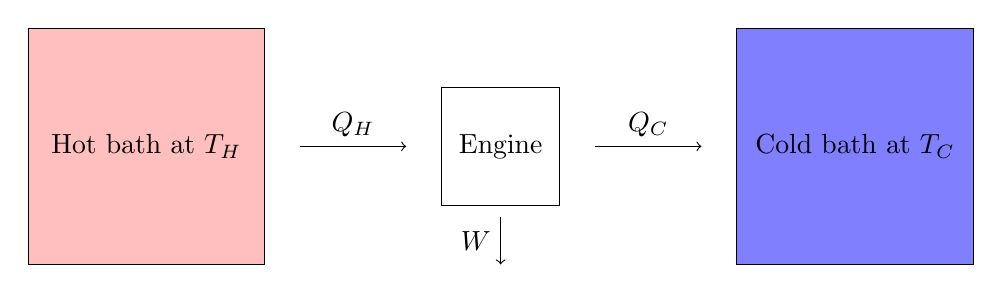
\begin{tikzpicture}[scale=3]
    \filldraw[fill=pink] (0,0) rectangle (1,1);
    \draw (1.75,0.25) rectangle (2.25,0.75);
    \filldraw[fill=blue!50] (3,0) rectangle (4,1);
    \draw[->] (1.15,0.5) -- (1.6,0.5);
    \draw[->] (2.4,0.5) -- (2.85,0.5);
    \draw[->] (2,0.2) -- (2,0);
    \node[above] at (1.375,0.5) {$Q_H$};
    \node[above] at (2.625,0.5) {$Q_C$};
    \node[left] at (2,0.1) {$W$};
    \draw (2,0.5) node {Engine};
    \draw (0.5,0.5) node {Hot bath at $T_H$};
    \draw (3.5,0.5) node {Cold bath at $T_C$};=
    \end{tikzpicture}
\end{center}


Now, let's consider the entropy of the hot reservoir, the engine, and the cold reservoir at the end of one cycle (in other words, we consider the change in entropy of the universe after one cycle). We recall that entropy is a function of state, and therefore at the end of a single cycle, the entropy of the heat engine itself must be the same as when it started. That is, $\Delta S_{engine} = 0$ for one full cycle. By the second law of thermodynamics $dS \geq \frac{Q}{T}$, the entropy of the hot reservoir decreases by the amount of heat $Q_H$ divided by its temperature $T_H$, so the entropy of the hot reservoir decreases by $\Delta S_{hot} \geq \frac{-Q_H}{T_H}$. Conversely, the cold reservoir increases in one cycle by $\Delta S_{cold} \geq \frac{Q_C}{T_C}$ (as it receives $Q_C$ heat at temperature $T_C$. Putting these together, we obtain the change in entropy of the universe for a single cycle:
\[\Delta S_{universe} \geq \frac{Q_C}{T_C} - \frac{Q_H}{T_H} \]
Now, the second law of thermodynamics tells us that the entropy of the universe must increase (or, to phrase it another way, if we treat the two reservoirs and the heat engine as an isolated system, the entropy of the total system must increase. This allows us to conclude that:
\[\Delta S_{universe} \geq \frac{Q_C}{T_C} - \frac{Q_H}{T_H} \geq 0 \]
So we obtain the important inequality:
\[\frac{Q_C}{T_C} - \frac{Q_H}{T_H} \geq 0 \]
Which we can rearrange to obtain:
\begin{equation}
    \label{eqn:(37)}
    \frac{T_H}{T_C} \geq \frac{Q_C}{Q_H}
\end{equation}
Note that to derive inequality \ref{eqn:(37)}, I have made no assumptions whatsoever about what my heat engine actually looks like; this is a completely general statement, based on the amounts of heat gained/lost from the hot/cold reservoirs, and the maximum/minimum hot/cold reservoir temperatures. Now, let us consider out definition of efficiency:
\begin{equation}
    \label{eqn:(38)}
    \eta = \frac{W}{Q_H}
\end{equation}
Where $W$ is the work done by the engine (what we get out), and $Q_H$ is the heat that we inject into the engine in one cycle from the hot reservoir (what we put in). By energy conservation, we find that:
\begin{equation}
    \label{eqn:(39)}
    W = Q_H-Q_C
\end{equation}
This might look like it came out of nowhere, so let's think about it a bit further. Just like entropy, internal energy is also a function of state; the energy something has doesn't care about how that energy got there! With this consideration, since the heat engine returns to the original state at the end of one cycle, just like the entropy change of the heat engine is zero in a single cycle, so must be the total internal energy; in other words, the heat engine must have the same energy it began with. With this consideration, we realize that the sum of the work done on the system and the heat given to the system must be 0, leading to equation \ref{eqn:(39)} above (work this out using the first law of thermodynamics if it's still unclear!). Now, we can substitute equation \ref{eqn:(39)} into equation \ref{eqn:(38)}, giving us:
\begin{align*}
    \eta = \frac{Q_H-Q_C}{Q_H} = 1 - \frac{Q_C}{Q_H}
\end{align*}
And now applying inequality \ref{eqn:(37)}, we have:
\begin{align*}
    1 - \frac{Q_C}{Q_H} \leq 1 - \frac{T_H}{T_C}
\end{align*}
And therefore:
\begin{equation}
    \eta \leq 1 - \frac{T_H}{T_C}
\end{equation}
We have hence proven Carnot's theorem, and can see that for any arbitrary heat engine, the efficiency is bounded by the Carnot efficiency. 

\subsection{The Statistical Definition of Entropy}
Entropy has a more fundamental definition (though that doesn't make the classical definition any less important) rooted in statistics. To understand it, we're going to start of my talking about macrostates and microstates.
\subsubsection{Macrostates and Microstates}
I'll try to define these two words as succinctly as I can.
\begin{itemize}
    \item Macrostate: The state of a system as characterized by quantities that can be measured independent of any one part of the system. Some examples of such quantities would be: Pressure, Volume, and Temperature.
    \item Microstate: The state of a system as characterized by the state of individual components of the system. For example, the exact spacial distribution of particles within a gas.
\end{itemize}
Let's look as a bit more of a concrete example. Say we're looking at a box with 6 particles, divided into two halves.

\begin{figure}[ht!]
    \centering
\begin{tikzpicture}
\draw[draw = black] (0,0) rectangle (6,3);
\draw[dashed] (3,0) -- (3,3);
\draw[fill=red, draw=red] (1,2) circle (2pt);
\draw[fill=blue, draw=blue] (2,2) circle (2pt);
\draw[fill=cyan, draw=cyan] (1.5,1) circle (2pt);
\draw[fill=magenta, draw=magenta] (4,1) circle (2pt);
\draw[fill=orange, draw=orange] (5,1) circle (2pt);
\draw[fill=green, draw=green] (4.5,2) circle (2pt);
\end{tikzpicture}
    \caption{The box with three particles on each side.}
\end{figure}
\phantom{i} \\
\phantom{i} \\
The \textit{macrostate} of this box is something we could say without knowing which particle was where. Without knowing that, all we could say is that each side of the box has three particles. So, the macrostate of the box is three particles on each side. The \textit{microstate} of the box would then be which exact side each particle was on. So for example...

\begin{figure}[ht!]
    \centering
\begin{tikzpicture}
\draw[draw = black] (0,0) rectangle (6,3);
\draw[dashed] (3,0) -- (3,3);
\draw[fill=red, draw=red] (1.5,1.5) circle (2pt);
\draw[fill=blue, draw=blue] (5,1) circle (2pt);
\draw[fill=cyan, draw=cyan] (4.5,1.5) circle (2pt);
\draw[fill=magenta, draw=magenta] (4,2) circle (2pt);
\draw[fill=orange, draw=orange] (4,1) circle (2pt);
\draw[fill=green, draw=green] (5,2) circle (2pt);
\end{tikzpicture}
    \caption{This box has a different number of particles on each side, so it's in as different \textit{macrostate} than the first one.}
\end{figure}
\begin{figure}[ht!]
    \centering
\begin{tikzpicture}
\draw[draw = black] (0,0) rectangle (6,3);
\draw[dashed] (3,0) -- (3,3);
\draw[fill=red, draw=red] (1,2) circle (2pt);
\draw[fill=orange, draw=orange] (2,2) circle (2pt);
\draw[fill=cyan, draw=cyan] (1.5,1) circle (2pt);
\draw[fill=magenta, draw=magenta] (4,1) circle (2pt);
\draw[fill=blue, draw=blue] (5,1) circle (2pt);
\draw[fill=green, draw=green] (4.5,2) circle (2pt);
\end{tikzpicture}
    \caption{This box has the same number of particles on each side, so it's the same \textit{macrostate} as the first one. However, the blue and orange particles have switched sides, making this a different \textit{microstate} than the first box had. Note that two different macrostates of a system cannot share a microstate.}
\end{figure}
\newpage



\subsubsection{The Definition of Entropy}
Now that we know what micro and macro states are, we can define entropy using statistics! In this case, entropy is defined as
\begin{equation}
    \label{eqn:(41)}
    S=k_{b}\ln{\Omega}
\end{equation}

where $\Omega$ is the number of possible microstates within the current macrostate of the system. \\
With a closed system of constant volume, we can characterize macrostates using the temperature of the system, and microstates as the exact distribution of kinetic energies amongst the particles in the system. Using this we can start to see all the parallels between the two different ways of defining entropy.
\begin{enumerate}
    \item At $T=0\textrm{K}$ every particle must have no kinetic energy. So, there's only one possible microstate, and by equation \ref{eqn:(41)} above $S=0$. This is exactly what we'd expect from the third law of thermodynamics, at absolute zero temperature, we obtain that entropy has a constant value\footnote{Note that the third law of thermodynamics does not say a system reaches zero entropy as it approaches zero temperature, as there do exist certain systems where the minimum energy (i.e. low temperature) states are not unique. Therefore, there still can be more than one microstate, and hence nonzero (but still constant) entropy. You don't need to know about these in any kind of detail.}.
    \item If you have two systems (a and b), the amount of microstates in a system including both of them is $\Omega_{a}\Omega_{b}$. Therefore, the total entropy is...
    \begin{align*}
        S_{total}&=k_{b}\ln{\Omega_{a}\Omega_{b}} \\
        &=k_{b}\ln{\Omega_{a}}+k_{b}\ln{\Omega_{b}} \\
        &=S_{1}+S_{2}
    \end{align*}
    Since the total entropy is the sum of the entropy of both systems, entropy is an extensive quantity!
    \item In our example for microstates/macrostates above, the macrostate with the highest number of microstates was the one where each side had three particles (if you don't believe me count them). This analogy applies to two systems that can exchange energy, they have the maximum number of microstates (and therefore entropy) when they share the energy equally (i.e. have the same temperature). 
\end{enumerate}
To close off our discussion of macrostates, microstates, and the statistical definition of entropy, let us consider another concrete example, in the form of the entropy of rolling two dice. Therein, we can consider the macrostate as the sum of the two dice rolls, and the microstates as the particular values we got on each dice (here, we imagine that the dice are unique, in that I can tell them apart from each other). For example, if I rolled the first dice to be 6, and the second dice to be 1, then the microstate could be described with $(6,1)$ and this microstate belongs to the macrostate of $7$. A complete description of all of the macrostates and microstates (as well as the entropy of the macrostate, as defined in this section) is given in the table below, though you may want to work this out for yourself first for practice.

\begin{center}
 \begin{tabular}{|c c c|} 
 \hline
 \textbf{Macrostates} & \textbf{Microstates} & \textbf{Entropy}\\ 
 \hline\hline
 2 & (1,1) & $k_b\ln(1) = 0$\\ 
 \hline
 3 & (1,2),(2,1) & $k_b\ln(2)$ \\
 \hline
 4 & (1,3),(2,2),(3,1) & $k_b\ln(3)$ \\
 \hline
 5 & (1,4),(2,3),(3,2),(4,1) & $k_b\ln(4)$ \\
 \hline
 6 & (1,5),(2,4),(3,3),(4,2),(5,1) & $k_b\ln(5)$ \\
 \hline
 7 & (1,6),(2,5),(3,4),(4,3),(5,2),(6,1) & $k_b\ln(6)$\\
 \hline
 8 & (2,6),(3,5),(4,4),(5,3),(6,2) & $k_b\ln(5)$\\
 \hline
 9 & (3,6),(4,5),(5,4),(6,3) & $k_b\ln(4)$\\
 \hline
 10 & (4,6),(5,5),(6,4) & $k_b\ln(3)$\\
 \hline
 11 & (5,6),(6,5) & $k_b\ln(2)$\\
 \hline
 12 & (6,6) & $k_b\ln(1) = 0$\\
 \hline
\end{tabular}
\end{center}
This example also demonstrates an assumption I implicitly made up until this point: all possible microstates are equally likely to appear (in the last example, unless you had loaded dice, every dice roll would have been equally likely!). This is a very fundamental assumption, so much so that it is called the \textbf{Fundamental Assumption of Statistical Mechanics}. Just to restate it for a more general case (as not every system in the universe is a bunch of dice), it states that every microstate of a system is equally likely and the system on average spends the same amount of time in each of them. We will use this in the next section to conclude our discussion of entropy. 
\subsubsection{The Arrow of Time}
One interesting property of a lot of physics equations is that they are invariant under time reversal; that is, equations like Newton's second law 
\begin{align*}
\vec{F} = m\vec{a}
\end{align*}
can be applied even in cases where time was running in reverse\footnote{Assuming no friction, of course.}. However, it is clear in our immediate experience that a lot of things are not invariant under time reversal. If I were to show you a video of heat flowing from a cold bath of water to a hot bath of water, you would tell me immediately that the video must be playing in reverse. If the laws of physics are supposed to work the same way in either direction, what's going on here?

As we discussed previously, where we see phenomena that only proceed in one time direction, what we are seeing is something go from a low entropy state to a higher entropy state. After the process, by the second law of thermodynamics, we can't go back to the lower entropy state. But this explanation feels a bit unsatisfactory; sure, we've accepted the second law of thermodynamics as a law, but there's still this underlying feeling of "Well, why \textbf{can't} things go back to a lower entropy state?" The statistical definition will allow us to settle this confusion once and for all.

From a statistical viewpoint, what are we saying when a system goes from a low to a high entropy state? Well by the definition of $S = k_b\ln\mathbb{W}$ for the entropy of a macrostate, what we're really saying is that the system moves from a macrostate with a low number of microstates to a high number of microstates. Okay sure, but why? Well let's think back to the fundamental assumption of statistical mechanics that I just outlined a page ago. This assumption tells us that every microstate is equally as likely to appear, and each microstate persists for the same amount of time. Well, if every microstate is equally as likely, then simple notions of probability will tell us that the system at any given point will tend to a macrostate with more microstates.

Let's try to make this a little more concrete with an example. Say I was keeping tracks of 10 numbered cows in a field, separated into a left and right hand side, where the cows were allowed to walk around the field totally randomly. Then, a macrostate of the system could be defined by how many cows were on the left side of the field (where I have 11 microstates, from 0-10 cows on the left side). Now, suppose I start in a configuration where all 10 cows are on the left side of the field. There are a couple ways in which I could arrange the cows in this scenario. However, the macrostate corresponding to 5 cows on the right side and 5 cows on the left side of the field has a lot more microstates; there are a lot more ways I could arrange 5 and 5 cows on either side of the field compared to having all the cows on one side. With this in mind, let's imagine that the cows start all on one side, I walk away from the field, and come back some amount of time later after the cows were free to move around. Since every configuration of cows is equally likely, I would be most likely see a state where the cows were distributed equally on both sides of the field (as we would expect). Probabilistically, the system has evolved from an initial low entropy state (all cows on one side) to a higher entropy state (cows distributed on both sides).

Now, imagine instead of left and right side of a field, we have two containers of gas in thermal contact, which can freely exchange units of energy (which have replaced the cows in this scenario). Although now we have an extremely large number of energy units instead of just 10\footnote{Many 10s of orders of magnitude more...}, the same sort of logic applies; if I start in a macrostate with all of the energy units on one side (i.e. one gas container is very hot, and the other is not), with time, the system will tend to a macrostate of thermal equilibrium (approximately equal thermal energy on either side) as there are so many more microstates for the equilibrium temperature macrostate compared to a macrostate where one side has a lot more energy units than the other. Hence, we have come up with a statistical explanation for why heat tends to flow from hot objects to cold objects!

Note that this analysis reveals something interesting about the second law of thermodynamics; it's very much a statistical law, that tells us that a isolated system is (extremely) likely to tend to a high entropy state. Note that both in the cows and the heat example, there technically is a possibility that the system could temporarily return to a low entropy state (either with all the cows, or all the thermal energy units on one side); its just that this configuration is \textbf{extremely unlikely}. In fact, as we make our system larger and larger, the likelihood that the system could ever return to a low entropy state becomes more and more unlikely, and therefore in the limit of large/macroscopic systems, we can treat the second law as (basically) absolute. 

This concludes our discussion of Science One Thermodynamics. If you enjoyed this part of the course, I would highly recommend taking PHYS 203 (Thermal Physics) next year, even if you decide not to go into a physics major\footnote{If you do go into physics, you won't have a choice!}. If you go into chemistry, you will also cover more thermodynamics material in the CHEM 205+304 sequence. Schroeder's "An Introduction to Thermal Physics" is a good text to consult for further reading on the subject (if you wanted to go beyond the material covered in your textbooks this year). We hope that even if you found this unit challenging at times, you can appreciate how we can learn so much about the workings of the universe from a couple (fairly simple) definitions and laws; if not, we hope that you take pride in the fact that you've made it through one of the most difficult units of Science One physics!


\subsection{Practice Problems}
\begin{enumerate}
    \item What is the change in entropy of a system undergoing an adiabatic\footnote{For anyone going on to take 203, in this question we would also technically have the qualifier that the process was also \textbf{quasistatic}, but this is not relevant for our discussion here!} process? (Hint: return to the classical definition).
    \item Consider a situation where you are determining the entropy of rolling three (unique/distinguishable) dice. Consider the macrostate $7$, where $7$ is the sum of the three dice. What is the entropy of this macrostate?
    \item How does the answer to the above question change if you consider three indistinguishable dice? In this case, (1,1,2) and (1,2,1) would be the same, for example.
    \item What is the change in entropy of the gas medium of \textbf{any} heat engine after one cycle? Why?
    \item Explain using macrostates/microstates why if I remove a partition between two different gases in a box, why they will mix irreversibly and will never return to their original state. 
    \item Suppose I have a one mole of monoatomic gas of volume $V = 1m^3$ and temperature $T = 300K$. I first (isochorically) heat it up to $T=400K$, then I let it expand isothermally so that it is double its original size. What is the change in entropy of the gas (Hint: Use equation 34)?
    \item Imagine we have two compartments of gas separated by a movable piston (that is initially locked in place), initially located in the center. The two containers cannot exchange heat with each other (nor with their surroundings), and have the same initial volume $V$ and amount of gas $n$. Now assume that, initially, the temperature of the gas in the piston on the right hand side ($T_R$) is higher than that on the left ($T_L$). 
    \begin{enumerate}
        \item When I unlock the piston, what happens?
        \item What is the change in internal energy and entropy of the whole system?
        \item What can you say of the pressure, volume, and temperature on both sides at the end? Will the system be at thermal equilibrium?
    \end{enumerate}  
    
    \begin{center}
        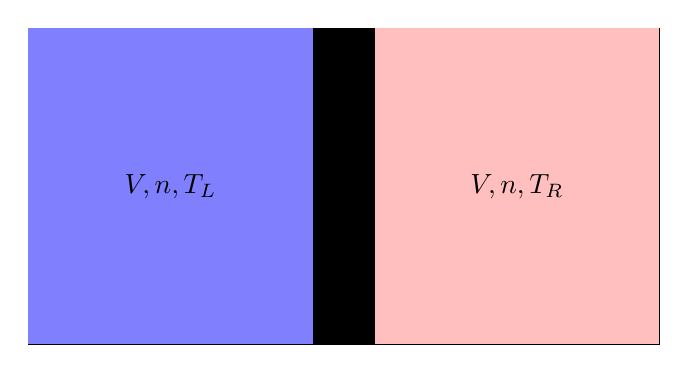
\begin{tikzpicture}[scale=4]
        \draw[black, thick] (0,0) rectangle (2,1);
        \filldraw[fill = black, draw = black] (0.9,0) rectangle (1.1,1);
        \filldraw[fill = blue!50, draw = blue!50] (0,0) rectangle(0.9,1);
         \filldraw[fill = pink, draw = pink] (1.1,0) rectangle(2,1);
        \draw[black] (0.45,0.5) node {$V,n,T_L$};
        \draw[black] (1.55,0.5) node {$V,n,T_R$};
        
        \end{tikzpicture}
    \end{center}
\end{enumerate}